\def\paperRoman{I}
\documentclass[10pt,a4paper]{article}
\usepackage[margin=22mm,top=23mm,bottom=23mm]{geometry}
\usepackage{fontspec}
\setmainfont{Latin Modern Roman}
\setsansfont{DejaVu Sans}
\usepackage{babel}
\babelprovide[import,main]{spanish}
\usepackage{amsmath,amssymb}
\usepackage{unicode-math}
\setmathfont{Latin Modern Math}
\usepackage{graphicx,booktabs,longtable,array,enumitem,xcolor,fancyhdr,xurl,hyperref,tikz,microtype}
\usetikzlibrary{arrows.meta,positioning}
\definecolor{navy}{HTML}{17375C}
\definecolor{teal}{HTML}{0F8F86}
\definecolor{gold}{HTML}{B28B3C}
\hypersetup{colorlinks=true,linkcolor=navy,urlcolor=teal,citecolor=navy,pdfauthor={Juan Manuel Goenaga Castro}}
\setlength{\parindent}{0pt}
\setlength{\parskip}{5.2pt}
\linespread{1.07}
\setlist{nosep,leftmargin=1.5em,topsep=4pt}
\setlength{\headheight}{15pt}
\pagestyle{fancy}
\fancyhf{}
\fancyhead[L]{\sffamily\footnotesize GoToGym Quantum Research}
\fancyhead[R]{\sffamily\footnotesize Serie QAF audiovisual / \paperRoman}
\fancyfoot[L]{\sffamily\scriptsize Prepublicación metodológica / 22 de octubre de 2026}
\fancyfoot[R]{\sffamily\footnotesize\thepage}
\renewcommand{\headrulewidth}{0.4pt}
\newcommand{\papertitle}[3]{\begin{center}\sffamily\small\textcolor{teal}{MANUSCRITO #1 / ARQUITECTURA AUDIOVISUAL QAF}\par\vspace{9pt}{\huge\bfseries\textcolor{navy}{#2}}\par\vspace{7pt}{\large #3}\par\vspace{11pt}{\normalsize\bfseries Juan Manuel Goenaga Castro}\par\small GoToGym Quantum Research / Bogotá D.C., Colombia\par\small 22 de octubre de 2026 / Versión 1.0\end{center}\vspace{4pt}}
\newcommand{\status}[1]{\noindent\colorbox{navy!7}{\parbox{0.966\linewidth}{\small\textbf{Naturaleza del trabajo.} #1}}\par\vspace{6pt}}
\newcommand{\keywords}[1]{\textbf{Palabras clave:} #1.}
\newcommand{\R}{\mathbb{R}}
\newcommand{\C}{\mathbb{C}}
\newcommand{\tr}{\operatorname{Tr}}
\newcommand{\diag}{\operatorname{diag}}
\newcommand{\argmin}{\operatorname*{arg\,min}}
\newcommand{\argmax}{\operatorname*{arg\,max}}
\newcommand{\IP}{\mathcal{I}}
\newcommand{\sectionpage}[1]{\clearpage\section{#1}}
\newcommand{\compacttable}{\small\renewcommand{\arraystretch}{1.22}}
\emergencystretch=2em

\begin{document}
\papertitle{I}{Fundamentos de un sistema audiovisual QAF}{Representación relacional, decisión verificable y transferencia de evidencia}
\status{Propuesta de arquitectura y formalización, con comprobaciones algebraicas reproducibles. La transferencia al rendimiento audiovisual es una hipótesis de investigación.}
\begin{abstract}
Se propone un sistema que transforma conocimiento verificable en decisiones coordinadas de guion, imagen, voz, montaje y render. La contribución consiste en separar cuatro objetos que suelen confundirse: evidencia sobre el producto, estado de decisión, representación computacional y calidad percibida de la película. La propiedad intelectual QAF aportada se utiliza como antecedente para modelar relaciones, orden de intervenciones, compresión tensorial y compilación de decisiones. Se define una interfaz entre un grafo de evidencia y un espacio de alternativas; se especifican estados normalizados, observables y restricciones; y se presenta un mecanismo de admisión que exige utilidad incremental frente a un comparador clásico informado. Una prueba construida de cuatro estados muestra qué información de fase se pierde al conservar únicamente poblaciones, sin demostrar que esa información exista en una audiencia. Una enumeración independiente comprueba una formulación QUBO pequeña. El resultado es un programa falsable de desarrollo, con procedencia y límites explícitos, orientado a videos explicativos de 60 segundos.
\end{abstract}
\keywords{QAF, sistemas audiovisuales, evidencia, MPS, TDVP, RDM, QUBO, decisión multimodal}

\section{Problema, alcance y contribuciones}
La dificultad principal de una película explicativa no se reduce a producir imágenes atractivas. Un plano puede ser visualmente convincente y comunicar una capacidad inexistente; una locución puede ser clara y contradecir la demostración; un render puede ser correcto y exceder el presupuesto. El objeto de control es la relación entre decisiones de disciplinas diferentes. Se plantea la pregunta: \emph{¿puede una representación relacional mejorar comprensión, consistencia y eficiencia de producción frente a una planificación clásica que recibe las mismas fuentes, restricciones y recursos?}

El sistema se denomina aquí \textbf{QAF audiovisual}, como nombre de trabajo. No se presenta como producto desplegado, patente concedida o método cuya originalidad global haya sido establecida. Sus contribuciones propuestas son: un contrato de evidencia por afirmación y plano; una representación opcional del estado de decisión mediante redes tensoriales; una formulación combinatoria que conserva restricciones editoriales; y una regla de uso o rechazo basada en mediciones. El render físico y la síntesis de voz permanecen en motores especializados, desarrollados en los manuscritos III y IV.

La unidad mínima es un episodio de duración exacta, dirigido a una audiencia y una decisión comercial. El conocimiento se organiza en afirmaciones, no en un resumen indiscriminado de artículos. La meta de GoToGym, crear bienestar personalizado y hacerlo universalmente accesible, proporciona el propósito editorial; no sustituye la definición experimental de comprensión o utilidad.

\section{Procedencia de la propiedad intelectual y alcance de transferencia}
Los seis documentos suministrados desempeñan funciones distintas. El manuscrito técnico de septiembre de 2026 identifica a \textbf{Antoni Bancells} como autor; sus aportaciones se citan como antecedente y no se reasignan al autor de esta serie. Las nuevas propuestas y la integración audiovisual se preparan a nombre de Juan Manuel Goenaga Castro, conservando esa atribución.

\begin{table}[ht]\centering\compacttable
\begin{tabular}{p{.07\linewidth}p{.37\linewidth}p{.46\linewidth}}\toprule
Fuente & Aporte utilizado & Restricción de interpretación \\\midrule
Q1 & Campo, normalización, dinámica y decisión & Una demostración de tres estados no calibra una audiencia.\\
Q2 & MPS, TDVP, RDM, eventos y QUBO & Coste depende de enlace, topología e implementación.\\
Q3 & Comparadores y ablación contextual & Proxy de asignación; no benchmark de cine.\\
Q4 & Validación pequeña del motor completo & Recuperación de fase en un generador controlado.\\
Q5 & Criterios de uso y no uso & Exige comparador fuerte, generalización y presupuesto.\\
Q6 & Atlas e impacto por denominador & Cobertura del atlas no es éxito económico universal.\\\bottomrule
\end{tabular}\caption{Mapa de transferencia de los antecedentes aportados.}
\end{table}

En Q3 se reporta reducción de asignación a señuelos de 13,26\% a 6,11\%, dentro del banco sintético descrito. Ese resultado motiva estudiar relaciones; no autoriza anunciar una mejora equivalente en retención o ventas. Q4 reporta ARI medio 0,951 en su tarea de fase, con paridad frente al oráculo exacto. Q6 clasifica 22 de 45 condiciones como positivas y 18 como evidencia insuficiente: excluir estas últimas cambia el denominador. Estas cifras se registran como \emph{resultados reportados por las fuentes}, no como reproducciones de esta serie.

La cifra de 18,5 ms para 500 variables de Q2 no se adopta como tiempo de render ni latencia integral. Debe aislarse la operación efectivamente medida, distinguir compilación de resolución y registrar hardware, memoria asignada y pico total. Del mismo modo, un reordenamiento RCM es una heurística de ancho de banda; no garantiza una cota universal de dimensión de enlace ni resuelve de forma general el mínimo de ancho de banda.

\section{Contrato de evidencia y estado de decisión}
Sea $\mathcal E_t$ el conjunto de evidencias disponibles en el instante de producción $t$. Cada registro contiene identificador, origen, versión, fecha, entorno, alcance, permiso de uso y estado de verificación. Una afirmación $c$ debe enlazarse con uno o más registros y con el plano o segmento de voz donde aparecerá. Definimos una compuerta editorial binaria
\begin{equation}
 g_c=\mathbf 1\{\text{fuente pertinente, alcance compatible y verificación requerida completa}\}.
\end{equation}
$g_c$ es una decisión documental revisable; no una probabilidad de verdad. Una visualización conceptual puede ser válida como recurso si su rótulo y contexto impiden confundirla con una función disponible. La afirmación sobre disponibilidad continúa necesitando evidencia operacional.

El vector observable $z_t\in\R^p$ reúne presupuesto restante, duración, preferencias, incertidumbres y restricciones. Una normalización robusta se ajusta \emph{solo} sobre datos de entrenamiento o referencias fijadas, con máscara de ausencia $m_j$:
\begin{equation}
 \widetilde z_j=m_j\,\operatorname{clip}\!\left(\frac{z_j-a_j}{b_j-a_j},0,1\right),\qquad b_j>a_j.
\end{equation}
La ausencia no equivale a cero semántico; se conserva $m_j$ para distinguirla. Los intervalos y unidades se documentan. Euros, segundos, grados y calificaciones no se suman antes de normalizar o definir una utilidad con unidades consistentes.

Para alternativas discretas $x$, se propone una codificación explícita y contrastable
\begin{equation}
 \psi_\theta(x\mid z)=\sqrt{\pi_\theta(x\mid z)}\,e^{i\phi_\theta(x,z)},\quad
 \sum_x\pi_\theta(x\mid z)=1.
\end{equation}
La distribución $\pi_\theta$ representa alternativas del plan, no estados neuronales del espectador. La fase $\phi_\theta$ debe ser identificable mediante datos sobre orden y relaciones; asignarla a mano según la respuesta correcta produciría fuga de información. Si no existe esa identificación, se utiliza el modelo clásico sobre $z$ y su grafo.

El estado $\rho=|\psi\rangle\langle\psi|$ satisface $\rho\succeq0$ y $\tr\rho=1$. Una mezcla de hipótesis usa $\rho=\sum_h w_h\rho_h$, con $w_h\geq0$ y $\sum_h w_h=1$. Cuando se interpreta una lectura como probabilidad, se exige una POVM $\{E_a\}$:
\begin{equation}
 p(a\mid\rho)=\tr(E_a\rho),\qquad E_a\succeq0,\qquad\sum_aE_a=I.
\end{equation}
La suma arbitraria de utilidad marginal e interferencia no asegura positividad o normalización. Se conserva la información compleja como característica del modelo y se usa una lectura válida. La utilidad de una alternativa y su probabilidad de elección se calibran por separado.

\section{Representación tensorial y dinámica opcional}
Para $K$ decisiones con dimensión local $d$, la amplitud se escribe como MPS con fronteras abiertas:
\begin{equation}
 \psi(x_1,\ldots,x_K)=A^{[1]}_{x_1}A^{[2]}_{x_2}\cdots A^{[K]}_{x_K},\qquad
 A^{[k]}_{x_k}\in\C^{\chi_{k-1}\times\chi_k},\quad\chi_0=\chi_K=1.
\end{equation}
El almacenamiento es $O(Kd\chi^2)$ para enlace máximo $\chi$. Se obtiene economía únicamente cuando una aproximación útil mantiene enlaces moderados. Un estado general puede requerir enlace exponencial. MPS no equivale a resolver todo problema combinatorio en tiempo polinómico. La precisión se controla con peso singular descartado, error de observables y comparación en tamaños pequeños.

Sea $H(z_t,u_t)=H_0+\sum_r u_r(t)O_r$ un operador hermítico, con escala operacional $\hbar_{\mathrm{eff}}$ calibrada y sin interpretación física de Planck. La propuesta de evolución proyectada es
\begin{equation}
 \dot\psi=-\frac{i}{\hbar_{\mathrm{eff}}}P_{T_\psi\mathcal M_\chi}H\psi.
\end{equation}
El formalismo TDVP se apoya en Haegeman y colaboradores \cite{tdvp}. Las propiedades del flujo exacto no se atribuyen automáticamente al integrador numérico. Se registran error de norma, error local, convergencia con paso y deriva de energía cuando $H$ sea autónomo. Campos dependientes del tiempo no conservan necesariamente la energía.

El orden de decisiones puede representarse con mapas $\mathcal A$ y $\mathcal B$. Se contrasta $\mathcal B\circ\mathcal A(\rho)$ frente a $\mathcal A\circ\mathcal B(\rho)$ en casos emparejados. Los modelos clásicos recurrentes y los procesos parcialmente observables también pueden capturar efectos de orden. Por ello, $[A,B]\neq0$ es una propiedad del modelo, no una demostración de imposibilidad clásica.

Para incorporar olvido o revisión de evidencia se plantea, como extensión por validar, un generador de Lindblad con tasas no negativas, usando unidades con $\hbar_{\mathrm{eff}}=1$:
\begin{equation}
 \dot\rho=-i[H,\rho]+\sum_r\gamma_r\left(L_r\rho L_r^\dagger-\tfrac12\{L_r^\dagger L_r,\rho\}\right),\quad\gamma_r\geq0.
\end{equation}
No se impone este coste a episodios sencillos. Debe demostrarse primero que una dinámica añade valor frente a un estado estático o una memoria clásica.

\section{Observables, fase e identificabilidad}
Las matrices reducidas $\rho_a$ y $\rho_{ab}$ describen subsistemas del plan; se obtienen por traza parcial. Una característica candidata es
\begin{equation}
 \zeta_{ab}=\frac{\rho_{ab}[00,11]}{\sqrt{\rho_{ab}[00,00]\rho_{ab}[11,11]}},\qquad
 f_{ab}=(\Re\zeta_{ab},\Im\zeta_{ab}).
\end{equation}
La característica se omite si el denominador es inferior a un umbral fijado. Para una matriz positiva, $|\zeta_{ab}|\leq1$. La base, sus fases de referencia y la codificación se fijan antes del ajuste; una fase local arbitraria puede cambiar estas coordenadas. Una característica dependiente del gauge no se interpreta como significado humano universal.

En la prueba adjunta se construyen cuatro estados $\psi_\phi=(|00\rangle+e^{i\phi}|11\rangle)/\sqrt2$, con $\phi\in\{0,\pi/2,\pi,-\pi/2\}$. Sus diagonales son idénticas y $|\zeta|=1$ para todos. Una lectura compleja distingue los cuatro valores. Un clasificador constante sobre clases balanceadas obtiene 25\%; un clasificador por prototipos complejos, 100\%, \emph{en este conjunto construido y sin ruido}. La fidelidad máxima de rango uno frente al estado de Bell es $1/2$. Estos son controles algebraicos, no resultados de aprendizaje generalizable ni de comprensión audiovisual.

\begin{figure}[ht]\centering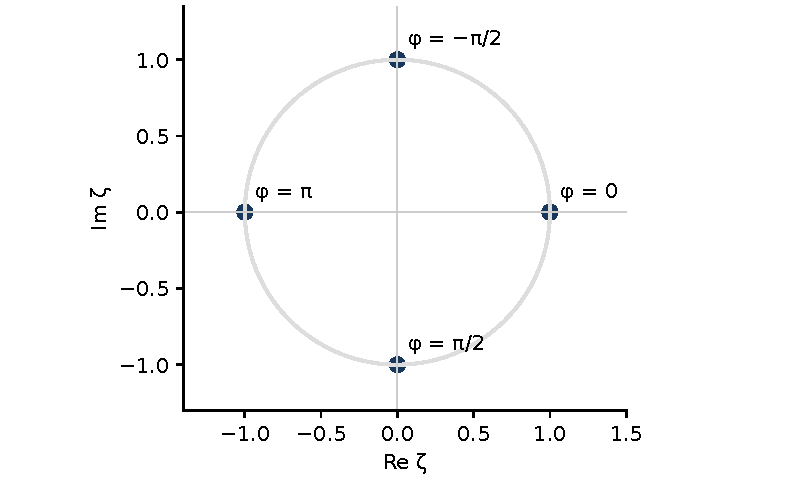
\includegraphics[width=.70\linewidth]{figures/phase_fixture.pdf}\caption{Característica compleja del ejemplo construido. El código fija la base y conoce la generación de los estados; no se aprende una fase a partir de espectadores.}\end{figure}

\section{Decisión restringida y compilación QUBO}
Sea $x_{ij}\in\{0,1\}$ la elección de variante $j$ para el plano $i$. La versión clásica minimiza coste editorial y de render bajo selección única, presupuesto y compatibilidad. Se formula primero de forma restringida; QUBO es una representación adicional que debe producir el mismo problema, no una excusa para cambiarlo \cite{bqm}.
\begin{align}
 \min_x\;&q^Tx+\sum_{a<b}v_{ab}x_ax_b,\\
 \text{sujeto a }&\sum_jx_{ij}=1,\quad c^Tx\leq B,\quad x_{ij}\leq g_{c(i,j)}.
\end{align}
El tiempo editorial se representa con cuadros enteros. Para 60 s y 30 fps, el presupuesto es 1.800 cuadros. Si se usan transiciones solapadas, sus cuadros se descuentan explícitamente; no se suman duraciones nominales como si no existiera solape.

Una igualdad de selección se penaliza mediante $\lambda_i(\sum_jx_{ij}-1)^2$. Presupuestos por desigualdad requieren holguras discretas acotadas o una formulación con restricciones nativas. La constante del QUBO se conserva al comparar energías. En la forma triangular $\sum_aQ_{aa}x_a+\sum_{a<b}Q_{ab}x_ax_b$, cada interacción aparece una vez. Si se usa matriz simétrica en $x^TQx$, los elementos no diagonales son la mitad del coeficiente triangular.

La prueba reproducible enumera 64 configuraciones de seis variables y ocho selecciones factibles. Con $B_0=\sum|q_a|+\sum|v_{ab}|$, se elige $\lambda>2B_0$ para que una violación entera no compense el rango del coste base. El mínimo penalizado coincide con el mínimo factible y con la versión simétrica. El resultado verifica la compilación de esa instancia, no la escalabilidad del sistema.

\section{Disparo por eventos y contratos de implementación}
Se recompila cuando cambia una evidencia material, una restricción o un observable por encima de tolerancia. Una condición propuesta combina desplazamiento de estado y novedad de grafo:
\begin{equation}
 \text{replanificar}\iff\tfrac12\|\rho_t-\rho_{t^-}\|_1>\tau_\rho\ \lor\ \Delta\mathcal E_t>\tau_E\ \lor\ \text{restricción nueva}.
\end{equation}
La distancia exige espacios de estado compatibles; un cambio de codificación o dimensión obliga a invalidar la comparación. El cambio de una afirmación crítica invalida los planos dependientes aunque la distancia del estado sea pequeña. Los umbrales son parámetros de control, no constantes científicas.

Los servicios propuestos son: ingesta de fuentes; compilador de afirmaciones; planificador editorial; motor relacional opcional; solucionador de restricciones; render especializado; revisión y publicación. Cada salida contiene versión de esquema, fuentes, decisiones, incertidumbres y recursos consumidos. Un plan aprobado es inmutable; una revisión genera otra versión con diferencias y motivo. Las claves de caché incluyen modelos, semilla, color, fuente, licencia y activos, además de la línea de tiempo.

\section{Criterio de aceptación, límites y conclusión}
QAF solo se admite si las cuatro compuertas de Q5 se verifican en el dominio: señal relacional pertinente, mejora sobre comparador clásico igualmente informado, resistencia a cambios de distribución y viabilidad computacional. Se rechaza cuando la fase no es identificable, el mejor comparador empata o supera el resultado, o el crecimiento de $\chi$ elimina la economía. La variante sencilla continúa siendo una solución válida del sistema.

La contribución de este manuscrito es una arquitectura verificable para coordinar decisiones audiovisuales y una colección de controles matemáticos. No demuestra calidad cinematográfica mundial, aumento de ventas ni ventaja cuántica. La evaluación humana, el render y el casting descritos en los otros manuscritos son experimentos necesarios para pasar de formalismo a capacidad profesional.

\begin{thebibliography}{Q6}
\bibitem[Q1]{q1} Goenaga, J. M. (2025). \emph{Quantum Analysis Frameworks}. Documento aportado, 4 pp.
\bibitem[Q2]{q2} Bancells, A. (2026). \emph{QAF: dinámica operacional no conmutativa y compilación QUBO asíncrona}. Manuscrito aportado, 15 pp.
\bibitem[Q3]{q3} Goenaga, J. M. (2026). \emph{Validación preliminar del QAF mediante benchmarking computacional reproducible}. 27 pp.
\bibitem[Q4]{q4} Goenaga, J. M. (2026). \emph{Validación end-to-end del motor QAF: MPS + TDVP + 1-RDM/2-RDM}. 17 pp.
\bibitem[Q5]{q5} Goenaga, J. M. (2026). \emph{Consolidated Experimental Evidence for QAF: When QAF Should and Should Not Be Used}. 8 pp.
\bibitem[Q6]{q6} Goenaga, J. M. (2026). \emph{Value and Non-Value Regions of QAF}. 8 pp.
\bibitem[E1]{tdvp} Haegeman et al. (2011). Time-dependent variational principle for quantum lattices. \emph{Phys. Rev. Lett. 107}, 070601. \url{https://arxiv.org/abs/1103.0936}.
\bibitem[E2]{bqm} D-Wave Quantum. Models: binary quadratic models. Documentación primaria, consulta 22/10/2026. \url{https://docs.dwavequantum.com/en/latest/concepts/models.html}.
\end{thebibliography}
\end{document}
